\subsection{Diagramme de Séquence}

le diagramme de séquence est un diagramme d’interaction qui expose en détail
la façon dont les opérations sont effectuées: quels messages sont envoyés et quand ils le sont. Les diagrammes de séquences sont organisés en fonction du temps qui s’écoule au fur et à mesure que nous parcourons la page. Les objets impliqués dans l’opération sont répertoriés de gauche, à droite en fonction du moment où ils prennent part dans la séquence.


%\begin{figure}
%	\centering
%	\includegraphics[width=0.7\linewidth]{mama/images/séquence}
%	\caption{}
%	\label{fig:sequence}
%\end{figure}

\begin{minipage}{0,8\textwidth}
	\includegraphics[width=0.7\linewidth]{mama/images/séquence}
\end{minipage}
\hspace*{\stretch{1}}


\subsection*{Diagramme de classes}

Le diagramme de classes exprime la structure statique du système en termes de classes et de relations entre ces classes. L’intérêt du diagramme de classe est de modéliser les entités du système d’information.
Le diagramme de classe permet de représenter l’ensemble des informations finalisées qui sont gérées par le domaine. Ces informations sont structurées, c’est-à-dire qu’elles sont regroupées dans des classes. Ce
diagramme met en évidence d’éventuelles relations entre ces classes.

\begin{minipage}{1\textwidth}
	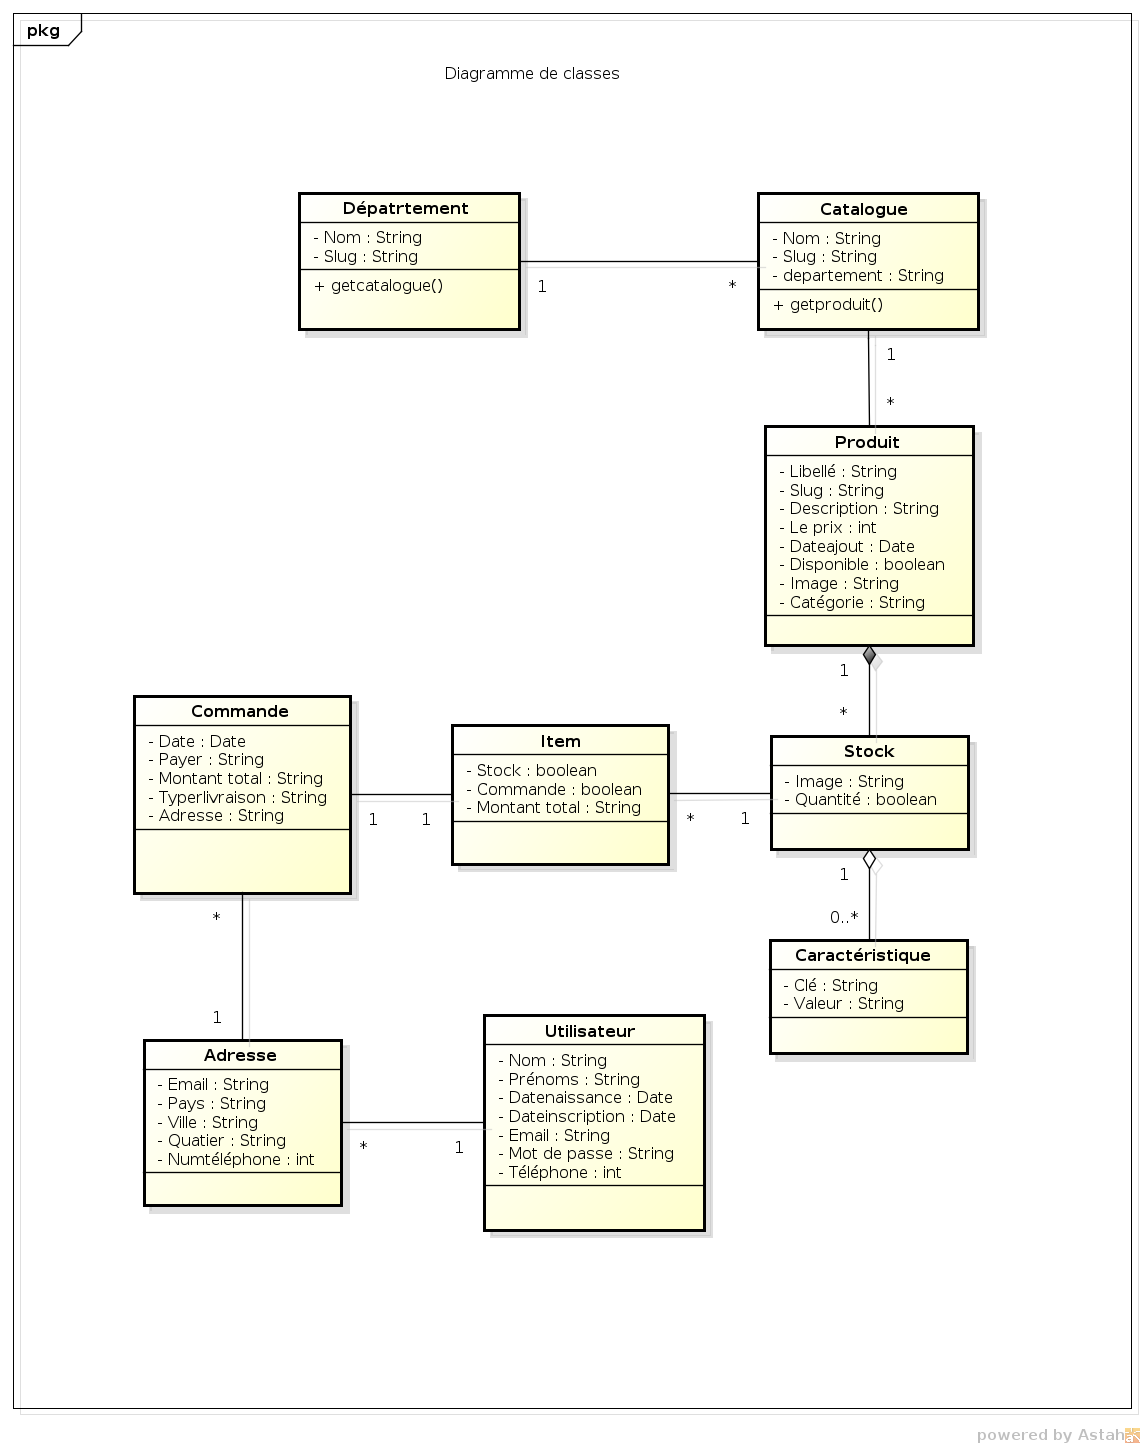
\includegraphics[width=0.7\linewidth]{mama/images/classes}
\end{minipage}
\hspace*{\stretch{1}}


 Chaque classe se décrit par les données et les traitements dont elle est responsable pour elle-même et vis-à-vis des autres classes. Les traitements sont matérialisés par des opérations.
